\documentclass[submit]{harvardml}

\course{CS181-S20}
\assignment{Assignment \#5}
\duedate{11:59pm April 10, 2020} 
\newcommand{\attr}[1]{\textsf{#1}}
\usepackage[OT1]{fontenc}
\usepackage[colorlinks,citecolor=blue,urlcolor=blue]{hyperref}
\usepackage[pdftex]{graphicx}
\usepackage{subfig}
\usepackage{fullpage}
\usepackage{amsmath}
\usepackage{amssymb}
\usepackage{color}
\usepackage{todonotes}
\usepackage{listings}
\usepackage{common}
\usepackage{bm}
\usepackage{enumitem}
\usepackage{tikz}
\usepackage{xifthen}
\usepackage{soul}

\usepackage[mmddyyyy,hhmmss]{datetime}

\definecolor{verbgray}{gray}{0.9}

\lstnewenvironment{csv}{
  \lstset{backgroundcolor=\color{verbgray},
  frame=single,
  framerule=0pt,
  basicstyle=\ttfamily,
  columns=fullflexible}}{}

\begin{document}
\begin{center}
{\Large Homework 5: Mixtures, EM, and Graphical Models}\\
\end{center}

This homework assignment will have you work with mixtures, EM, and
graphical models.  

Please type your solutions after the corresponding problems using this
\LaTeX\ template, and start each problem on a new page.

Please submit the \textbf{writeup PDF to the Gradescope assignment `HW5'}. Remember to assign pages for each question.

Please submit your \textbf{\LaTeX\ file and code files to the Gradescope assignment `HW5 - Supplemental'}. 

You can use a \textbf{maximum of 2 late days} on this assignment.  Late days will be counted based on the latest of your submissions. 
\\

\begin{problem}[Expectation-Maximization for Categorical-Geometric Mixture Models, 25pts]

In this problem we will explore expectation-maximization for a
Categorical-Geometric Mixture model.  Each observation $\boldx_n$ is a
positive integer scalar drawn from a geometric distribution
(associated with the number of trials needed to get to the first
success, if success occurs with probability $p$).  We posit that each
observation comes from \emph{one} mixture component.  For this
problem, we will assume there are $K$~components. Each component $k
\in \{1, \ldots, K\}$ will be associated with a probability $p_k \in
    [0,1]$.  Finally let the (unknown) overall mixing proportion of
    the components be~$\btheta \in [0,1]^K$, where~${\sum_{k=1}^K
      \btheta_k=1}$.

Our generative model is that each of the~$N$ observations comes from a
single component.  We encode observation $n$'s component-assignment as
a one-hot vector~${\boldz_n \in \{0,1\}^K}$ over components. This
one-hot vector is drawn from~$\btheta$; then, $\boldx_n$ is drawn
from~$\text{Geometric}(p_k )$ where $\boldx_n$ belongs to class $k$.

Formally, data are generated in two steps (assuming $\boldz_n$ encodes
the class $k$), where we define the PMF of the geometric distribution to be $p(x_n | p_k) = (1 - p_k)^{x_n - 1} p_k$:
\begin{eqnarray*}
 \boldz_n &\sim& \text{Categorical}(\btheta) \\
 \boldx_n &\sim& \text{Geometric}(p_k )
\end{eqnarray*}

  \begin{enumerate}

  \item \textbf{Intractability of the Data Likelihood} We are
    generally interested in finding a set of parameters $p_k$ that
    maximize the data likelihood $\log
    p(\{\boldx_n\}^N_{n=1}|\{p_k\}^K_{k = 1})$.  Expand the data
    likelihood to include the necessary sums over observations
    $\boldx_n$ and latents $\boldz_n$.  Why is optimizing this loss
    directly intractable?

\item \textbf{Complete-Data Log Likelihood} Define the complete data
  for this problem to be $D = \{(\boldx_n, \boldz_n)\}_{n=1}^N$. Write
  out the complete-data negative log likelihood. Note that optimizing
  this loss is now computationally tractable if we know $\boldz_n$.

\[\mcL(\btheta, \{p_k\}^K_{k=1}) =  -\ln p(D \given\btheta, \{p_k\}^K_{k=1}).\]


\item \textbf{Expectation Step} Our next step is to introduce a
  mathematical expression for $\boldq_n$, the posterior over the
  hidden topic variables~$\boldz_n$ conditioned on the observed data
  $\boldx_n$ with fixed parameters, i.e $p(\boldz_n | \boldx_n;
  \btheta, \{ p_k \}^K_{k=1})$.

\begin{itemize}
\item  \textbf{Part 3.A } Write down and simplify the expression for $\boldq_n$.
\item  \textbf{Part 3.B } Give an algorithm for calculating the expression for $\boldq_n$ found in Part 3.A for all $n$, given the observed data~$\{\boldx_n\}^N_{n=1}$ and settings of the parameters~$\btheta$ and~$\{ p_k\}^K_{k=1}$.

\end{itemize}

\item \textbf{Maximization Step}
Using the~$\boldq_n$ estimates from the Expectation Step, derive an update for maximizing the expected complete data log likelihood in terms of~$\btheta$ and~$\{ p_k \}^K_{k=1}$.

\begin{itemize}
    \item \textbf{Part 4.A } Derive an expression for the expected complete-data log likelihood using $\boldq_n$.
    \item \textbf{Part 4.B } Find an expression for $\btheta$ that maximizes this expected complete-data log likelihood. You may find it helpful to use Lagrange multipliers in order to enforce the constraint $\sum \theta_k = 1$. Why does this optimized $\btheta$ make intuitive sense?
    \item \textbf{Part 4.C } Apply a similar argument to find the
      values of $\{p_k \}^K_{k = 1}$ that maximizes the expected
      complete-data log likelihood.
\end{itemize}

\item Suppose that this had been a classification problem. That is,
  you were provided the ``true'' categories $\boldz_n$ for each observation $\boldx_n$,
  and you were going to perform the classification by
  inverting the provided generative model (i.e. now you're predicting $z$ given $x$). Could you reuse any of
  your inference derivations above?

\item Finally, implement your solution (see \texttt{T5\_P1.py} for starter code).  You are responsible for implementing the \texttt{loglikelihood}, \texttt{e\_step} and \texttt{m\_step} functions. Test it out with data given
  $10$ samples from $3$ components with $p_1 = .1$, $p_2=.5$, and
  $p_3=.9$.  How does it perform?  What if you increase the number of
  samples to $1000$ from each of the components?  What if you change
  $p_2=.2$?  Hypothesize reasons for the differences in performance
  when you make these changes. You may need to record five to ten trials (random restarts) in order to observe meaningful insights.

\end{enumerate}



\end{problem}

\subsection*{Solution}
\begin{enumerate}
    \item 
        \begin{equation}
            \begin{split}
                \log p(\{\boldx_n\}^N_{n=1}|\{p_k\}^K_{k = 1}) &= \log (\prod^N_{i=1} p(\{\boldx_n\}^N_{n=1}|\{p_k\}^K_{k = 1})\\
                &= \sum^N_{i=1} \log (p(\boldx_i|\{p_k\}^K_{k = 1}))\\
                &= \sum^N_{i=1} \log (p(\sum^K_{k=i}\boldx_i, \boldz_i = C_k|\{p_k\}^K_{k = 1}))\\
                &= \sum^N_{i=1} \log ( \sum^K_{k=i} p(\boldx_i \given \boldz_i = C_k, \{p_k\}^K_{k = 1})p(\boldz_i = C_k \given \{p_k\}^K_{k = 1}))\\
                &= \sum^N_{i=1} \log ( \sum^K_{k=i} \btheta_k(1-p_k)^{\boldx_n-1}p_k)
            \end{split}
        \end{equation}
        The summation of the latent variable inside the log makes optimizing this loss directly intractable.
    \item The negative log-likelihohod is given by:
        \begin{equation}
            \begin{split}
                \mcL(\btheta, \{p_k\}^K_{k=1}) &=  -\ln p(\{(\boldx_n, \boldz_n)\}_{n=1}^N \given\btheta, \{p_k\}^K_{k=1})\\
                &= - \sum^N_{n=1} \sum^K_{k=1} \boldz_{nk} \left(\ln ((1-p_k)^{x_n - 1}p_k) + \ln \btheta_k\right)
            \end{split}
        \end{equation}
    \item
        \begin{itemize}
            \item \textbf{Part 3.A }
                \begin{equation}
                    \begin{split}
                        \boldq_n = \mathbb{E} [\boldz_n \given \boldx_n] &= \left[p(\boldz_n \given \boldx_n; \btheta, p_n)\right] \\
                        &\propto \left[p(\boldx_n \given \boldz_n; p_k)  p(\boldz_n; \btheta)\right] \\
                        &\propto \left[\prod^K_{k=1}((1-p_k)^{x_n-1}p_k)^{z_{nk}}\prod^K_{k=1}\btheta^{z_{nk}}_k\right]
                    \end{split}
                \end{equation}
            \item \textbf{Part 3.B}\\
            We want to update the $\boldq$ for each data point in each cluster.
                \begin{verbatim}
                for n in N:
                    for k in K:
                        prob_x = (((1-p[k])**(x[n]-1)) * p[k]) ** z[n][k]
                        prob_z = theta ** z[n][k]
                        q[n,k] = prob_x * prob_z
                        
                \end{verbatim}
        \end{itemize}
    \item 
        \begin{itemize}
            \item \textbf{Part 4.A}
                \begin{equation}
                    \begin{split}
                    \mathbb{E}_{\boldz_n \given \boldx_n}\left[ \log p(\boldX, \boldZ \given \btheta, p_k)\right] &= \mathbb{E}_{\boldz_n \given \boldx_n}\left[ \sum^N_{n=1}(\log p(\boldx_n \given \boldz_n) + \log p(\boldz_n))\right]\\
                        &= \sum^N_{n=1}\mathbb{E}_{\boldz_n \given \boldx_n}\left[\log ( \prod^N_{n=1} ((1-p_k)^{x_n-1}p_k)^{z_{nk}} + \log(\prod^K_{k=1} \btheta_k^{z_{nk}})\right]\\
                        &= \sum^N_{n=1}\mathbb{E}_{\boldz_n \given \boldx_n}\left[\sum^N_{n=1} ((1-p_k)^{x_n-1}p_k) \boldz_{nk} + \sum^K_{k=1} \btheta_k \boldz_{nk})\right]\\
                        &= \sum^N_{n=1}\left[ ((1-p_k)^{x_n-1}p_k) \boldq_{nk}\right] + \sum^K_{k=1} \left[\btheta_k \boldq_{nk})\right]\\
                        &= \sum^N_{n=1} \sum^K_{k=1} \boldq_{nk} \left((1-p_k)^{x_n-1}p_k + \btheta_k\right)
                    \end{split}
                \end{equation}
            \item \textbf{Part 4.B}\\
                First, we take the derivative w.r.t. $\btheta$ and solve:
                \begin{equation}
                    \begin{split}
                        \log p(\boldX, \boldZ \given \btheta, p_k) &= \sum^N_{n=1} \sum^K_{k=1} \boldq_{nk} \left((1-p_k)^{x_n-1}p_k + \btheta_k\right) + \lambda\left( (\sum^K_{k=1} \btheta_k) -1 \right)\\
                        &= \frac{\partial}{\partial \btheta}\left[\sum^N_{n=1} \sum^K_{k=1} \boldq_{nk} \left((1-p_k)^{x_n-1}p_k + \btheta_k\right) + \lambda\left( (\sum^K_{k=1} \btheta_k) -1 \right)\right]\\
                        &= \sum^N_{n=1}\frac{\boldq_{nk}}{\btheta_k} + \lambda = 0 \\
                        \btheta_k &= \frac{-1}{\lambda}\sum^N_{n=1}\boldq_{nk}
                    \end{split}
                \end{equation}
                Now, we take the derivative w.r.t. $\lambda$ and solve:
                \begin{equation}
                    \begin{split} &=\frac{\partial}{\partial \lambda}\left[\sum^N_{n=1} \sum^K_{k=1} \boldq_{nk} \left((1-p_k)^{x_n-1}p_k + \btheta_k\right) + \lambda\left( (\sum^K_{k=1} \btheta_k) -1 \right)\right]\\
                    &= \sum^K_{k=1}\btheta_k=1\\
                    &= \sum^k_{k=1}\left(\frac{-1}{\lambda}\sum^N_{n=1}\boldq_{nk}\right)=1\\
                    \lambda &= - \sum^K_{k=1}\sum^N_{n=1}\boldq_{nk} = -N
                    \end{split}
                \end{equation}
                Now we can plug our expression for $\lambda$ back into our expression for $\btheta$:
                \begin{equation}
                    \hat{\btheta_k} = \frac{1}{N}\sum^N_{n=1}\boldq_{nk}
                \end{equation}
            This optimized $
            \btheta$ is intuitive because it shows that the most likely $\btheta_k$ for all $k \in \{1, \ldots, K\}$ is the average of the probabilities of each observation coming from component $k$ given the data point and all other known globals.
            \item \textbf{Part 4.C}
                \begin{equation}
                    \begin{split}
                    \mathbb{E}(\mcL) &= - \sum^N_{n=1} \sum^K_{k=1} \boldq_{nk} (\ln ((1-p_k)^{x_n - 1}p_k) + \ln \btheta_k)\\
                    \frac{\partial \mathbb{E}(\mcL)}{\partial p_k}&= \frac{q_{nk}}{(1-p_k)^{x_n-1}p_k}\left[(\boldx_n - 1)(1-p_k)^{x_n-2}p_k + (1-p_k)^{x_n-1}\right]\\
                    &= \frac{q_{nk}}{(1-p_k)^{x_n-1}p_k}\left[(\boldx_n - 1)(1-p_k)^{x_n}(1-p_k)^{-2}p_k + (1-p_k)^{x_n}(1-p_k)^{-2}(1-p_k)\right]\\
                    &= \frac{q_{nk}}{(1-p_k)^{x_n-1}p_k}\left[(1-p_k)^{x_n-2}\left((1-p_k)-p_k(\boldx_n-1)\right)\right]\\
                    &= \frac{q_{nk}}{(1-p_k)^{x_n-1}p_k}\left[(1-p_k)^{x_n-2}(1-p_k \boldx_n)\right]\\
                    &= \sum^N_{n=1}\frac{\boldq_{nk}(1-p_k)^{x_n-2}(1-p_k\boldx_n)}{(1-p_k)^{x_n-1}p_k}\\
                    0&= \sum^N_{n=1}\frac{\boldq_{nk}(1-p_k\boldx_n)}{(1-p_k)p_k}\\
                    &= \frac{1}{p_k(1-p_k)}\left(\sum^N_{n=1}\boldq_{nk} - \sum^N_{n=1}p_k\boldx_n\right)\\
                    \sum^N_{n=1}p_k\boldx_n &= \sum^N_{n=1}\boldq_{nk}\\
                    \hat{p_k} &= \frac{\sum^N_{n=1}\boldq_{nk}}{\sum^N_{n=1}\boldx_n\boldq_{nk}}
                    \end{split}
                \end{equation}
               $p$ is the probability of success for any one trial of the geometric random variable. In other words, $p_k$ represents 1 divided by a weighted average by the $q_{nk}$s of the number of trials required to get a success.  Intuitively this represents the probability of getting a success on any 1 trial
        \end{itemize}
    \item
        Yes, the only thing that would be different is you wouldn't have an expectation step. If you replace the $\boldq_{nk}$ with a one hot vector, you can reuse the EM.\\
    \item 
        There is no meaningful difference between the p values. The EM algo has a fair amount of variance and better performance with more data.
\end{enumerate}

\newpage

\begin{problem}[PCA, 15 pts]

For this problem you will implement PCA from scratch.  Using
\texttt{numpy} to call SVDs is fine, but don't use a third-party
machine learning implementation like \texttt{scikit-learn}.

We return to the MNIST data set from T4. You have been given
representations of 6000 MNIST images, each of which are $28\times28$
greyscale handwritten digits. Your job is to apply PCA on MNIST, and
discuss what kinds of structure is found.

As before, the given code in \texttt{T5\_P3.py} loads the images into your environment as a
6000x28x28 array.

\begin{enumerate}

\item Compute the PCA. Plot the eigenvalues corresponding to the most significant 500
  components in order from most significant to least. Make another plot that describes the cumulative proportion of variance explained by the first $k$ most significant components for values of $k$ from 1 through 500.
  How much variance is explained by the first 500 components?  Describe
  how the cumulative proportion of variance explained changes with $k$.

\item Plot the mean image as well as the images corresponding to the
  first 10 principle components.  How do the images compare to the
  cluster centers from K-means? Discuss any similarities and
  differences.

\item Compute the reconstruction error on the data set using the mean
  image. Then compute the reconstruction error using the first 10 principal components. How do these
  errors compare to the final objective loss achieved by using K-means on the dataset? Discuss any similarities and
  differences.

\end{enumerate}


\textit{Include your plots in your PDF. There may be several plots for this problem, so feel free
to take up multiple pages.}






\end{problem}


\subsection*{Solution}
\begin{enumerate}
    \item 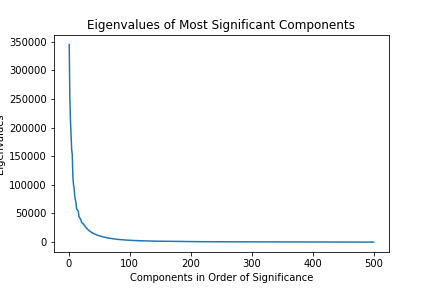
\includegraphics[]{EigSig (1).png}\\
    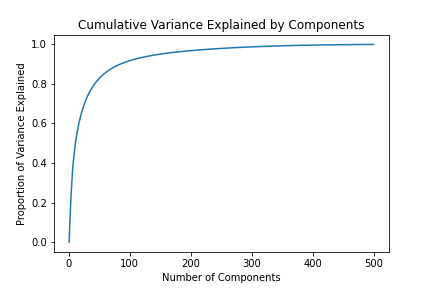
\includegraphics[]{VarExplained (1).png}\\
    \\
    
    \textbf{.9994 of variance} is explained by these first 500 components. \\
    We can see from this plot that close to .90 of the variance is explained by the first 50 components, so we do not really need 700+ variables to explain the vast majority of the variance.
    \item 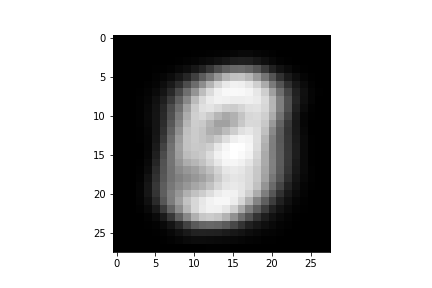
\includegraphics[scale = .5]{MeanImage (2).png}\\
    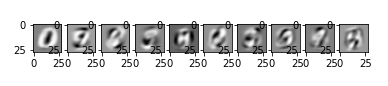
\includegraphics[]{FirstTenImg (1).png}\\
    The difference between PCA and K-means images is that the PCA images aren't supposed to represent the numbers themselves, but rather the components that explain the most variance. The K-means images were supposed to represent the digits themselves.
    \item The reconstruction error for the first ten principal components is: 7777920.42 \\
    
    The mean reconstruction error is: 11024181.87\\
    
    The K-Means final objective loss was around 9 million, so it was higher than the error for the first ten components but lower than the error for the mean.

\end{enumerate}
\newpage

\begin{problem}[Bayesian Networks, 10 pts]

  \noindent In this problem we explore the conditional independence
  properties of a Bayesian Network.  Consider the following Bayesian
  network representing a fictious person's activities. Each random
  variable is binary (true/false).

\begin{center}
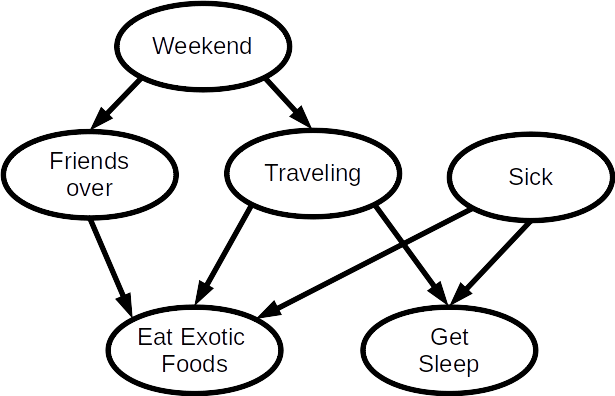
\includegraphics[width=2.5in]{bn.png}
\end{center}

The random variables are:

\begin{itemize}
\item \attr{Weekend}: Is it the weekend?
\item \attr{Friends over}: Does the person have friends over?
\item \attr{Traveling}: Is the person traveling?
\item \attr{Sick}: Is the person sick?
\item \attr{Eat exotic foods}: Is the person eating exotic foods?
\item \attr{Get Sleep}: Is the person getting sleep?
\end{itemize}

\medskip

For the following questions, $A \perp B$ means that events A and B are
independent and $A \perp B | C$ means that events A and B are independent
conditioned on C.

\textbf{Use the concept of d-separation} to answer the
questions and show your work (i.e., state what the blocking path(s) is/are and what nodes block the path; or explain why each path is not blocked).

\textbf{Example:} Is $\attr{Friends over} \perp \attr{Traveling}$? If NO, give intuition for why.

\textbf{Answer:} NO. The path from Friends over -- Weekend -- Traveling is not blocked following the d-separation rules. Thus, the two are not independent. Intuitively, this makes sense as if say we knew that the person was traveling, it would make it more likely to be the weekend. This would then make it more likely for the person to have friends over. 

\begin{enumerate}
\item Is $\attr{Sick} \perp \attr{Weekend}$?
  If NO, give intuition for why.


\item Is $\attr{Sick} \perp \attr{Friends over}\given \attr{Eat exotic
  foods}$? If NO, give intuition for why.


\item Is $\attr{Friends over} \perp \attr{Get Sleep}$? If NO, give
  intuition for why.

\item Is $\attr{Friends over} \perp \attr{Get Sleep} \given
  \attr{Traveling}$? If NO, give intuition for why.

\item Suppose the person stops traveling in ways that affect their
  sleep patterns (as various famous people have done).  Travel still
  affects whether they eat exotic foods.  Draw the modified network.

\item For this modified network, is $\attr{Friends over} \perp
  \attr{Get Sleep}$? If NO, give an intuition why.  If YES,
  describe what observations (if any) would cause them to no longer be
  independent.

\end{enumerate}
\end{problem}


\section*{Solution}
\begin{enumerate}
    \item Yes because in each of the 4 paths, it is blocked. Also, if someone is sick, that doesn't make it more or less likely to be the weekend.\\
    
    \item No, because sick - eat - friends over is an unblocked path. This makes sense intuitively, because if we knew the person had friends over and was eating exotic foods, it would be less likely they were sick.\\
    
    \item No. The path from friends over - weekend - traveling - get sleep is not blocked. Intuitively this makes sense because, if say, we knew the person's sleep was affected, it would be more likely they were traveling, which would make it more likely it is the weekend. This would then make it more likely to affect whether that person has friends over.\\
    
    Additionally, the path from weekend - traveling - get sleep is unblocked, which makes sense intuitively because if we observe it being the weekend but not that someone was traveling, it would be more likely that they are getting sleep. \\
    
    \item Yes. If getting sleep is conditioned on traveling, "friends - eating - travel - get sleep", "friends - weekend - travel - get sleep", and "friends - weekend - travel - eat - sick - and get sleep" are all blocked following d-separation rules. While "friends - eat - sick - get sleep" doesn't contain traveling, it is still blocked because friends over and sick are independent since we haven't observed E. \\
    
    \item 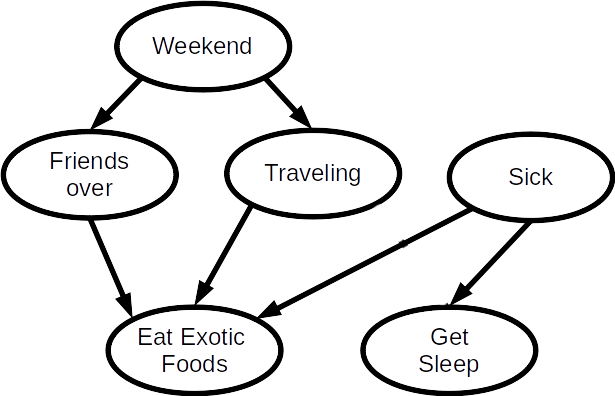
\includegraphics[scale = .5]{bnnew.png}\\
    
    \item Yes. The friends - eat - sick - get sleep path is blocked because friends over is independent of sick. The friends - weekend - traveling - eat - sick - get sleep path is blocked because traveling is independent of sick. If we were to observe the foods they ate, then they would no longer be independent.
    
\end{enumerate}

\newpage
%%%%%%%%%%%%%%%%%%%%%%%%%%%%%%%%%%%%%%%%%%%%%
% Name and Calibration
%%%%%%%%%%%%%%%%%%%%%%%%%%%%%%%%%%%%%%%%%%%%%
\subsection*{Name}

\subsection*{Collaborators and Resources}
Whom did you work with, and did you use any resources beyond cs181-textbook and your notes?

Office Hours

\subsection*{Calibration}
Approximately how long did this homework take you to complete (in hours)? 

~10 hours

\end{document}
